%\newcommand{\met}{\ensuremath{\mspace{3mu}/\mspace{-12.0mu}E_{T}}} 


\begin{figure}[hbt]
\begin{center}
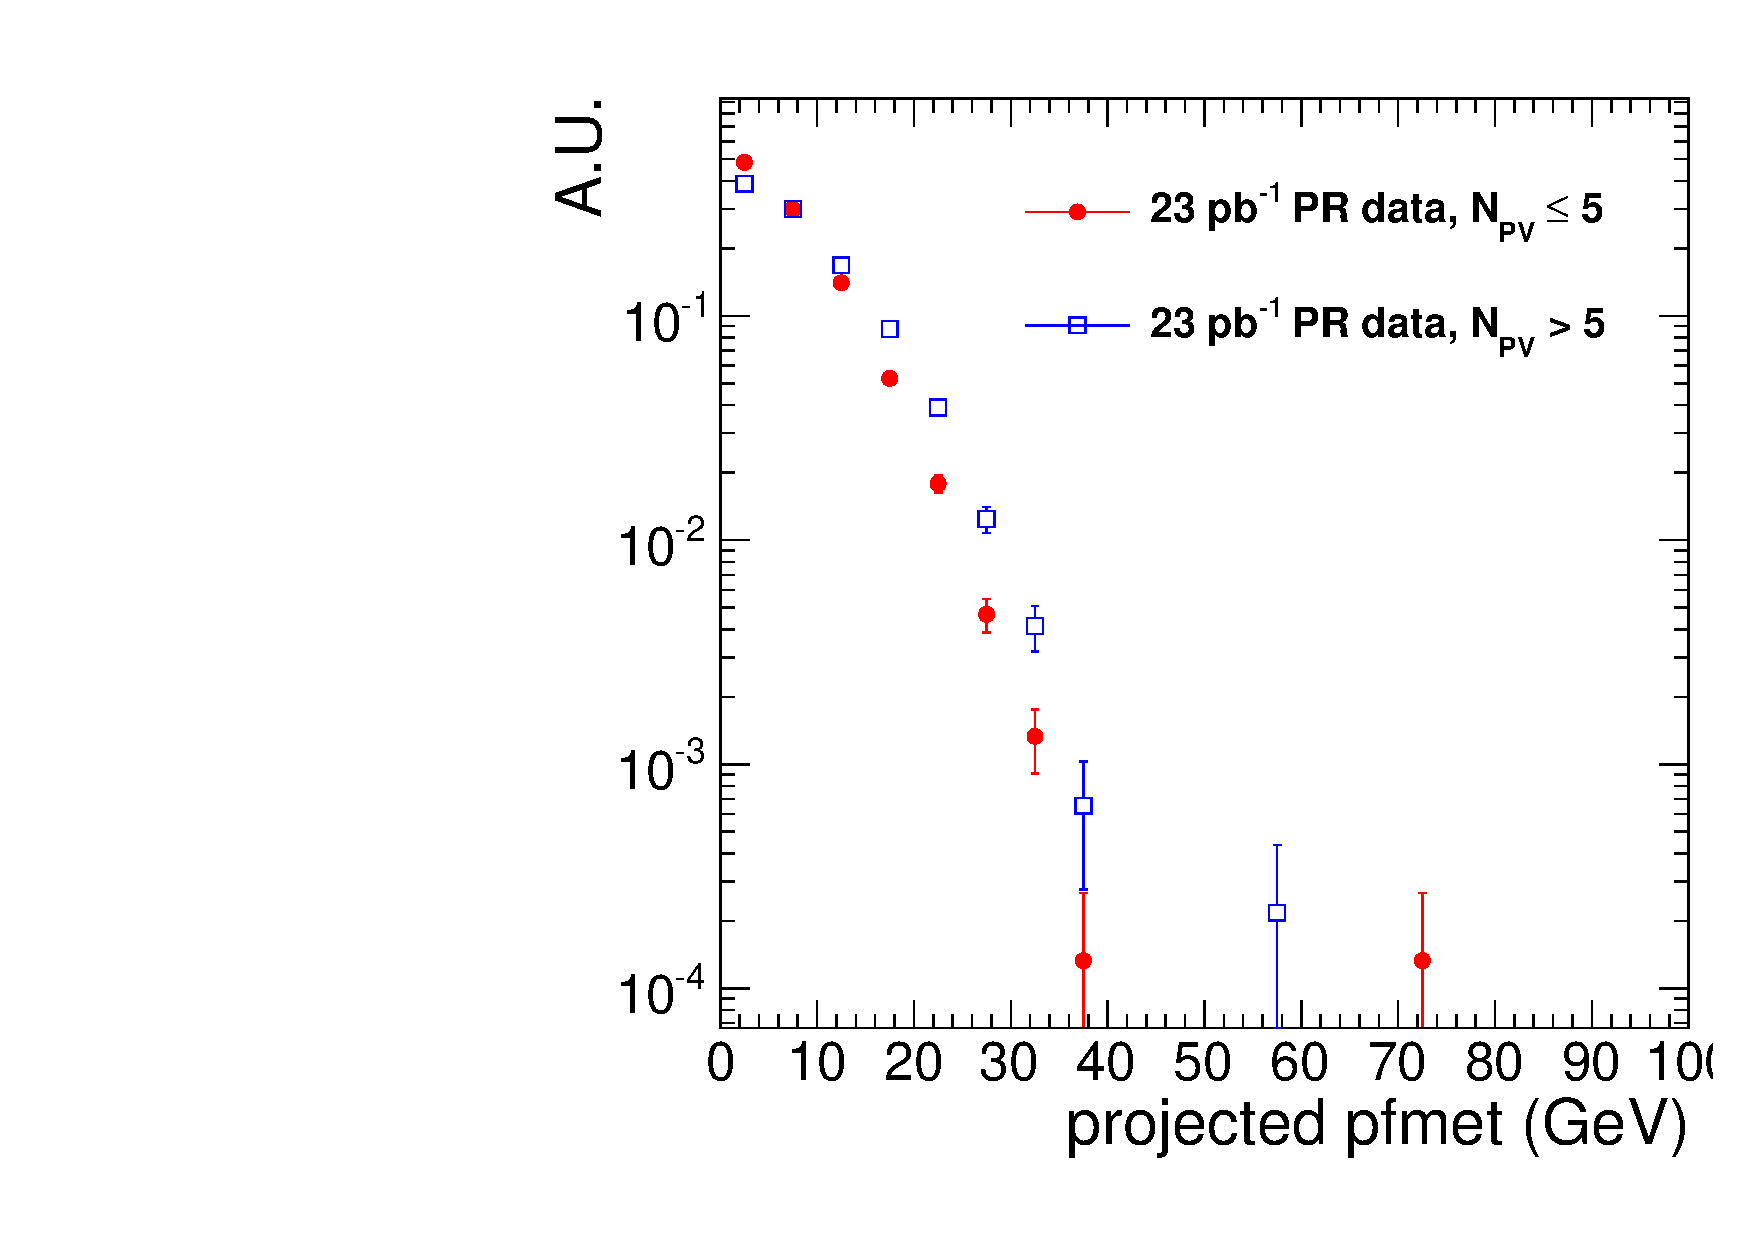
\includegraphics[width=0.3\linewidth]{figures/pfmet_data.pdf} 
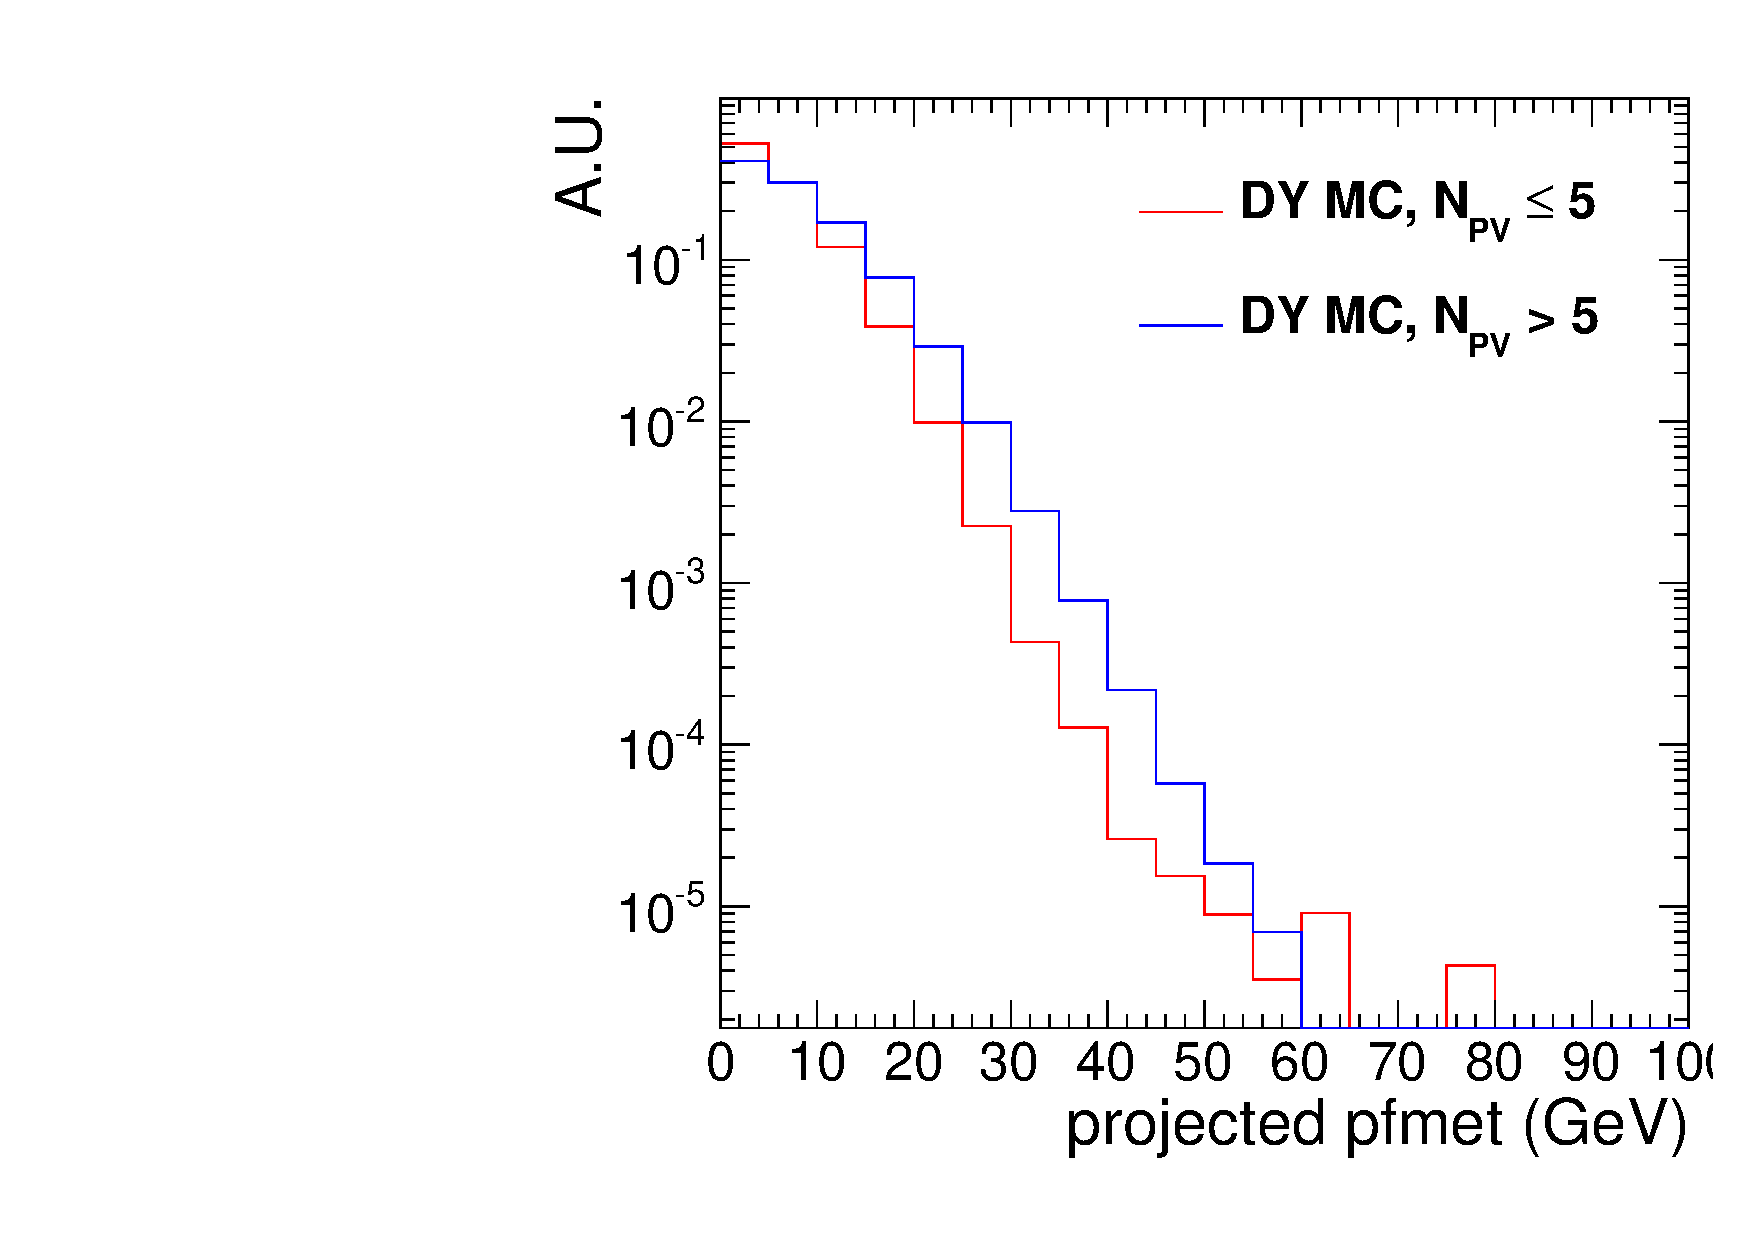
\includegraphics[width=0.3\linewidth]{figures/pfmet_dymc.pdf}
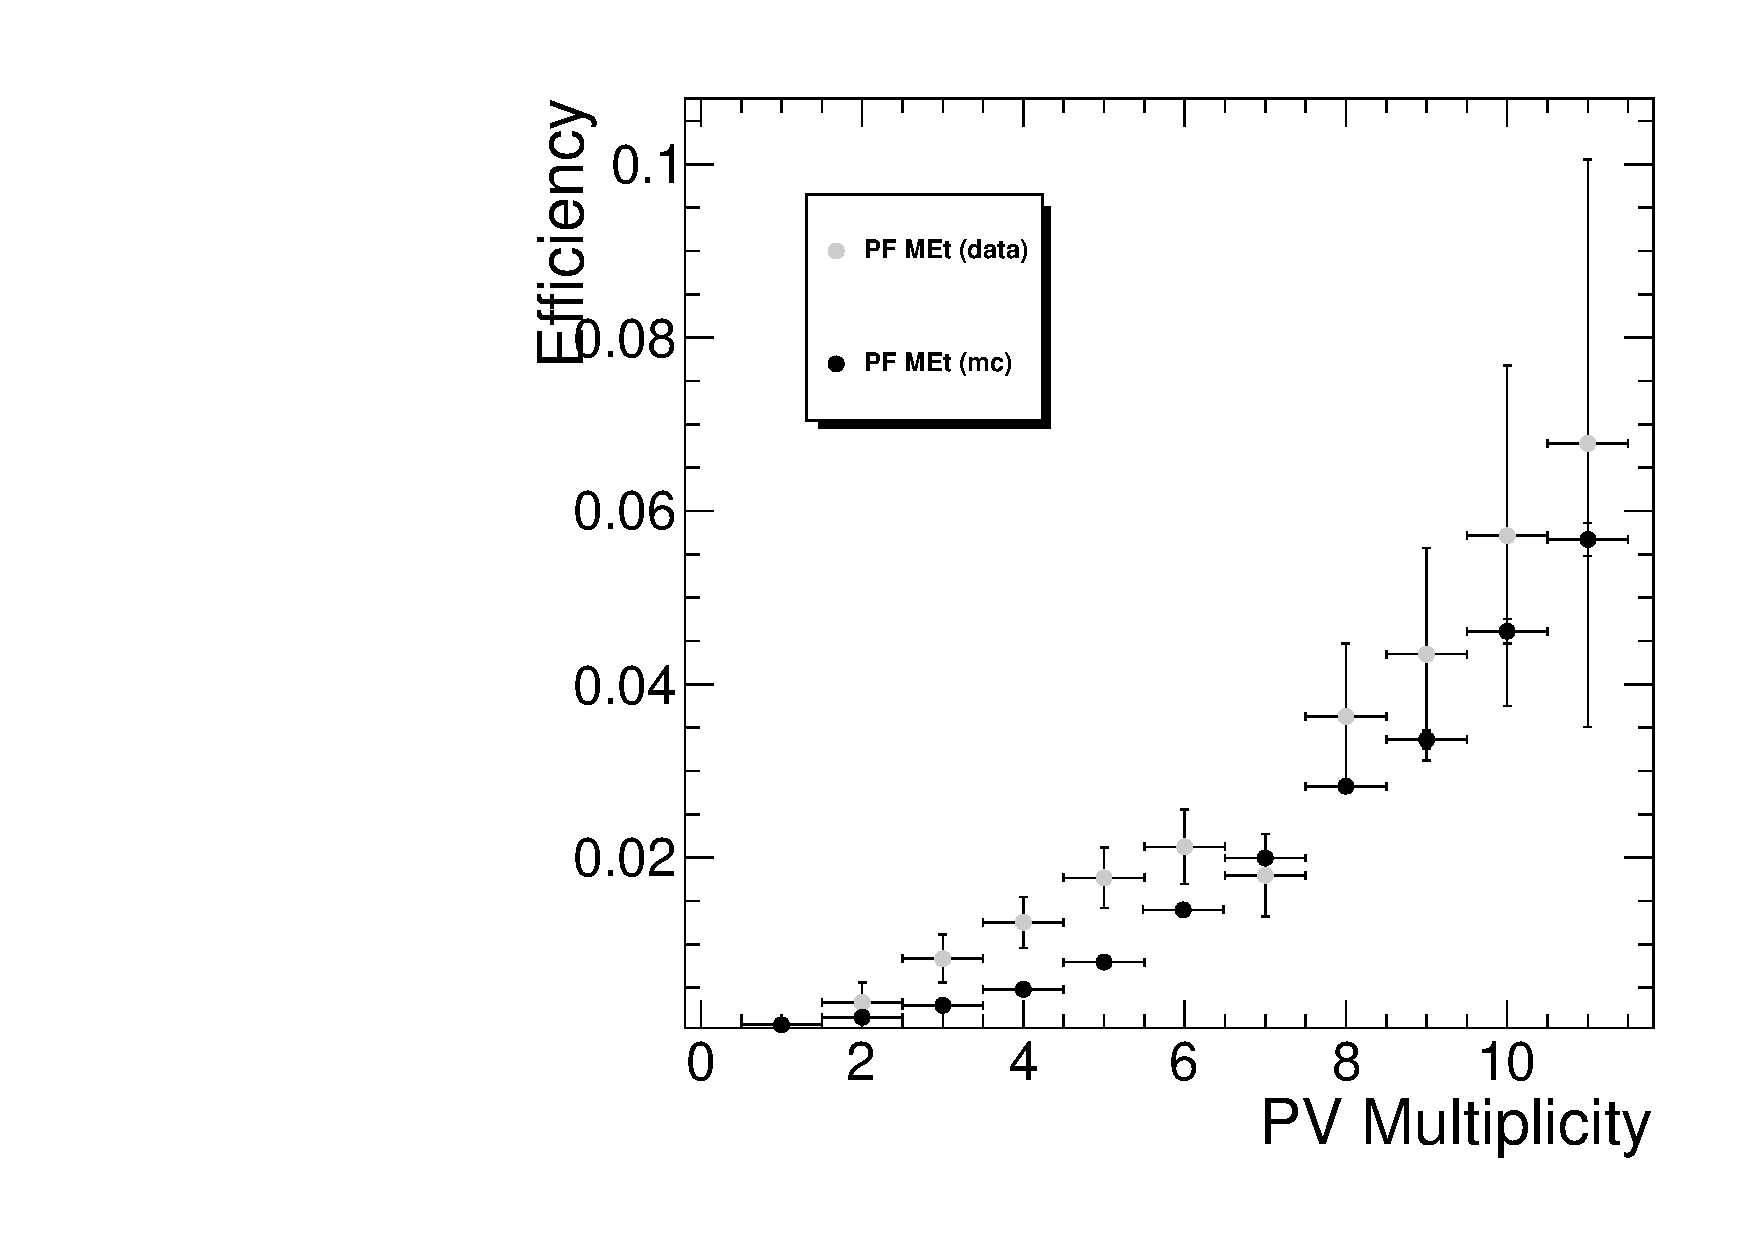
\includegraphics[width=0.3\linewidth]{figures/pfmet_Eff30.pdf} 
\caption{\label{fig:met_pu}\protect Distributions of pfmet in data (left) and DY MC (center) 
overlayed for low pile-up and high pile-up. The efficiency to satisfy the requirement pfmet$>30$~GeV as a function
of the number of reconstructed vertices in DY data and MC.}
\end{center}
\end{figure}

A requirement of large missing transverse energy (\met) is used to reject DY events.
In the presence of high pile-up, the instrumental \met\ tail in DY events is enhanced
significantly, as shown in Fig.~\ref{fig:met_pu} for data and DY MC. This causes a sharp increase in the
efficiency for DY events to pass a given \met\ requirement as the number of pile-up
interactions increases. To improve the robustness of the \met\ performance
in the presence of pile-up, we have developed a novel \met\ algorithm (trk-MET).
trk-MET is \met\ constructed from charged particles consistent with originating from
the signal PV. We correct for the 2 leptons, as well as charged PFCandidates which satisfy
the following requirements:
\begin{itemize}
\item the track matched to PFCandidate has $\delta z < 0.1$~cm with respect to the signal PV,
\item the signal PV is the closest PV to the track in $\delta z$, and
\item the track has $\Delta R > 0.1$ with respect to both leptons (to avoid double-counting of the leptons).
\end{itemize}
The high \met\ tail in events with no genuine \met\ is larger for trk-MET than for pfmet. However,
we observe that for data and MC DY events these two \met\ flavors are weakly-correlated, as shown
in Fig.~\ref{fig:met_scatter}. Therefore the rejection power for DY events is increased significantly
by cutting on both pfmet and trk-MET, or equivalently by cutting on min-MET $\equiv$ minimum(pfmet,trk-MET).
In addition, the high \met\ tail efficiency vs. number of pile-up interactions is flattened, as shown
in Fig.~\ref{fig:met_eff}. For signals with genuine \met\, trk-MET and pfmet are strongly correlated. 
The signal (H(130) MC) efficiency vs. background (DY MC) efficiency is shown in Fig.~\ref{fig:met_roc}
for min-MET and pfmet. For a DY background efficiency of $10^{-3}$, we observe a relative increase
in the signal efficiency of X\% (Y\%) for a number of pile-up interaction $<X$ ($<Y$).
 
\begin{figure}[hbt]
\begin{center}
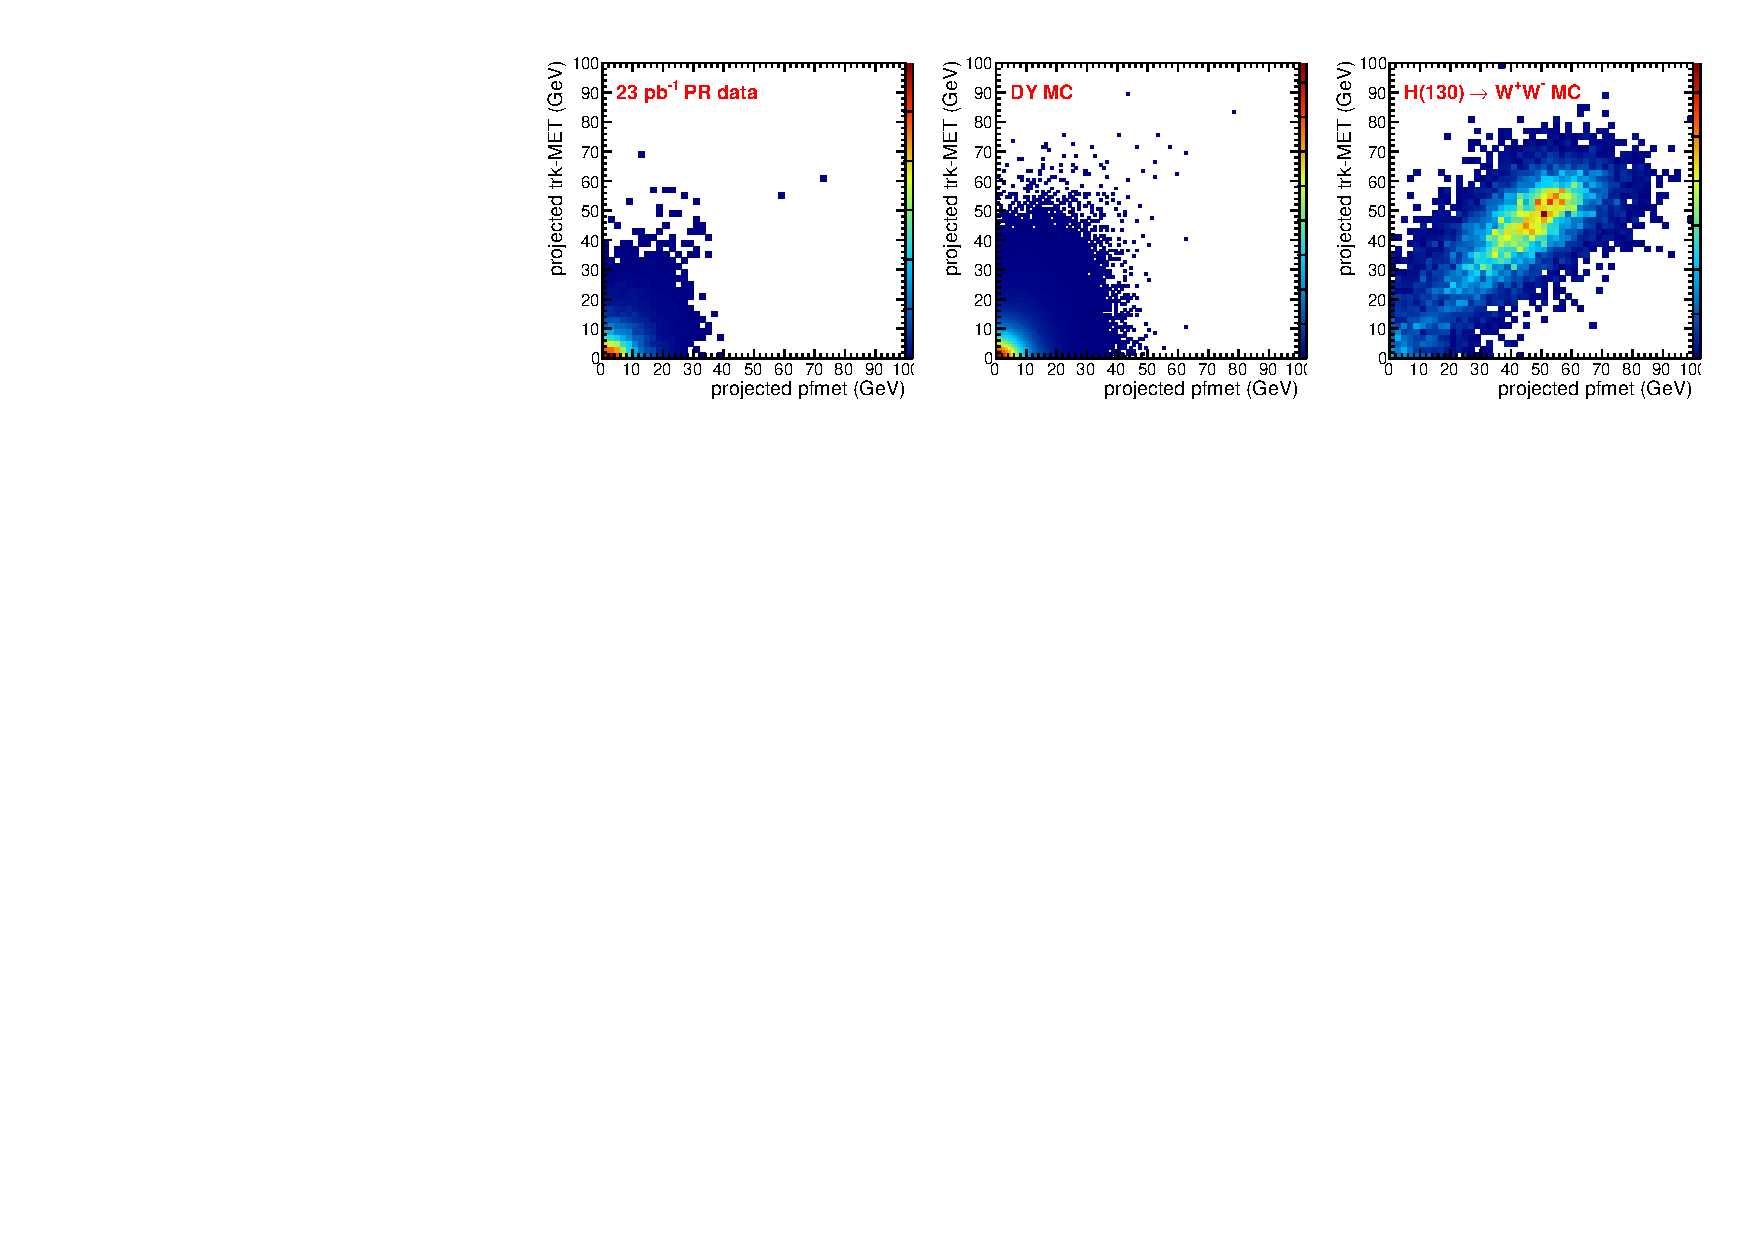
\includegraphics[width=1\linewidth]{figures/met_scatter.pdf} 
\caption{\label{fig:met_scatter}\protect Distributions of trk-MET vs. pfmet in data (left), DY MC (center) and Higgs MC (right).}
\end{center}
\end{figure}

 
\begin{figure}[hbt]
\begin{center}
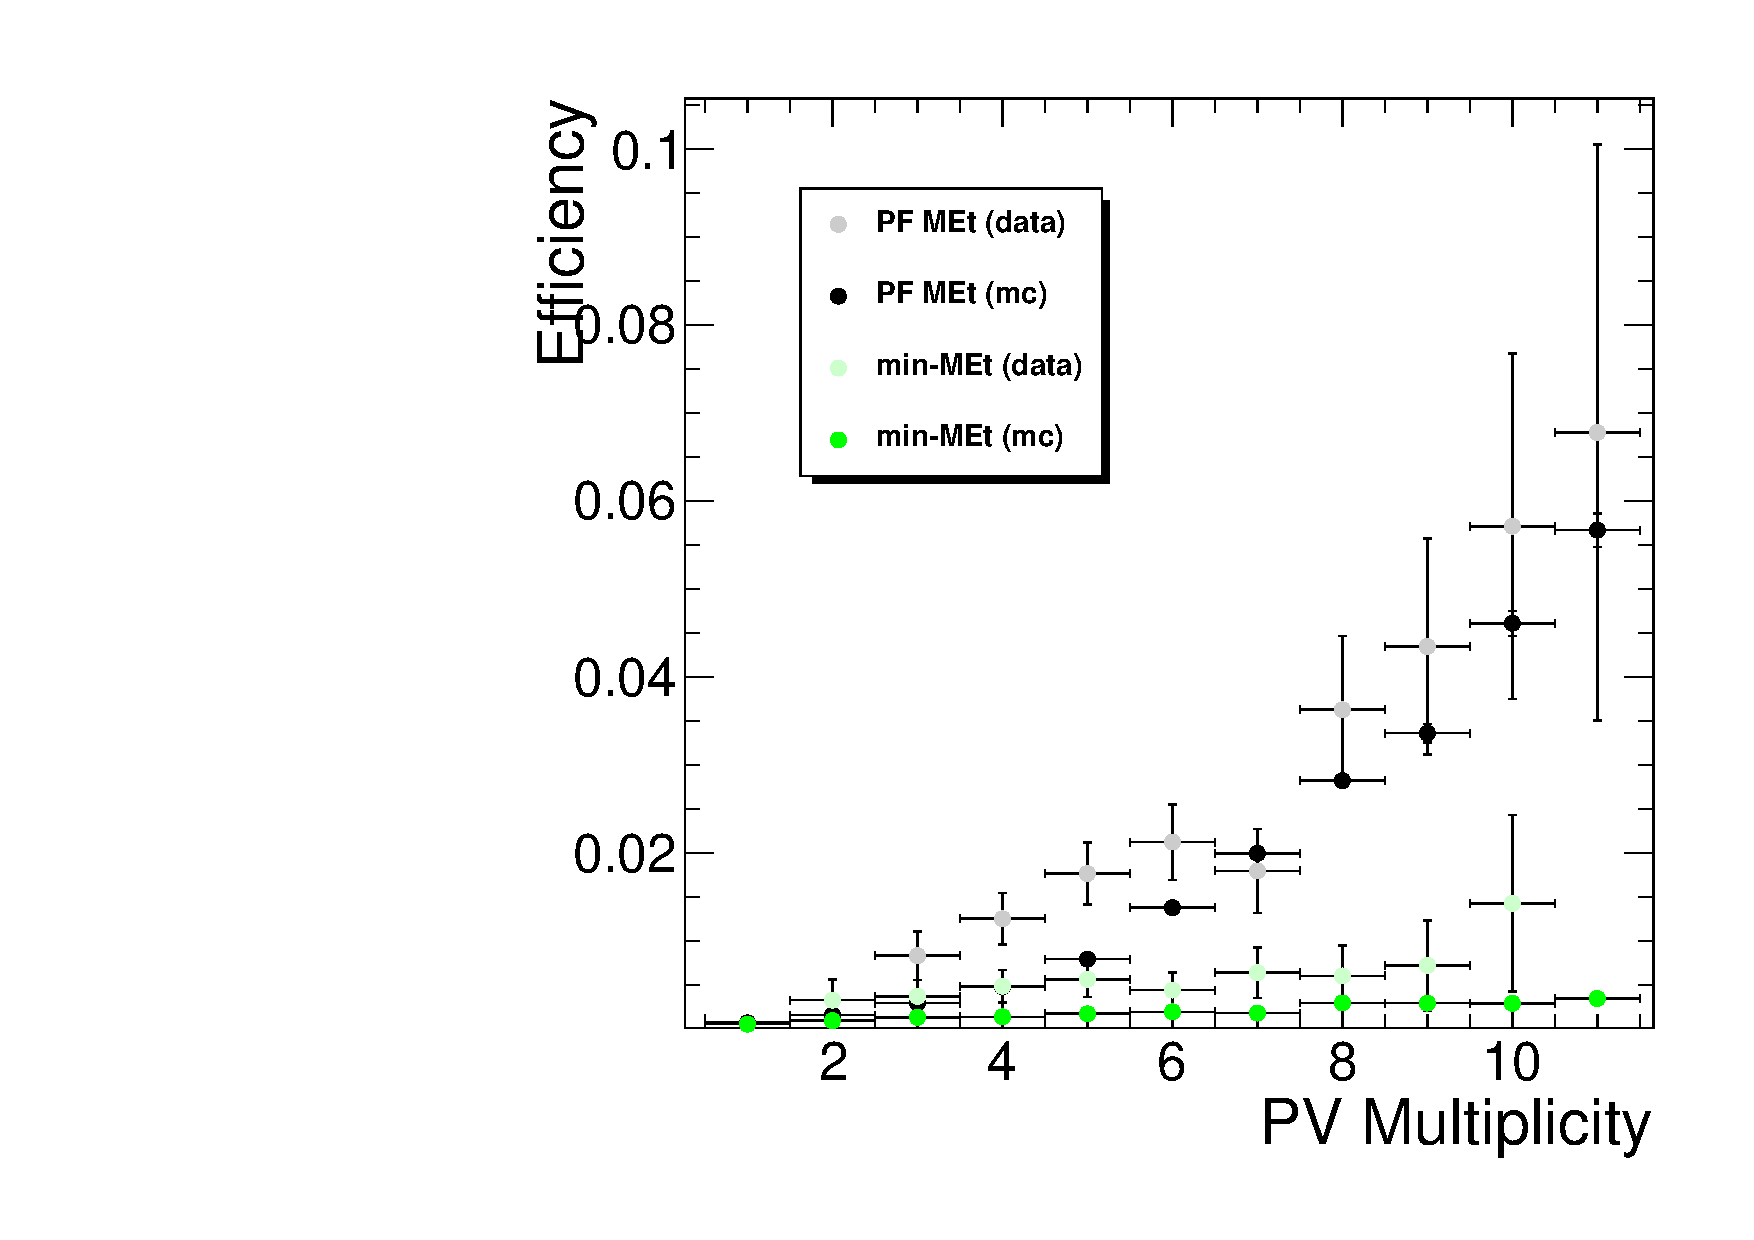
\includegraphics[width=0.45\linewidth]{figures/pfmet_minmet_Eff30.pdf} 
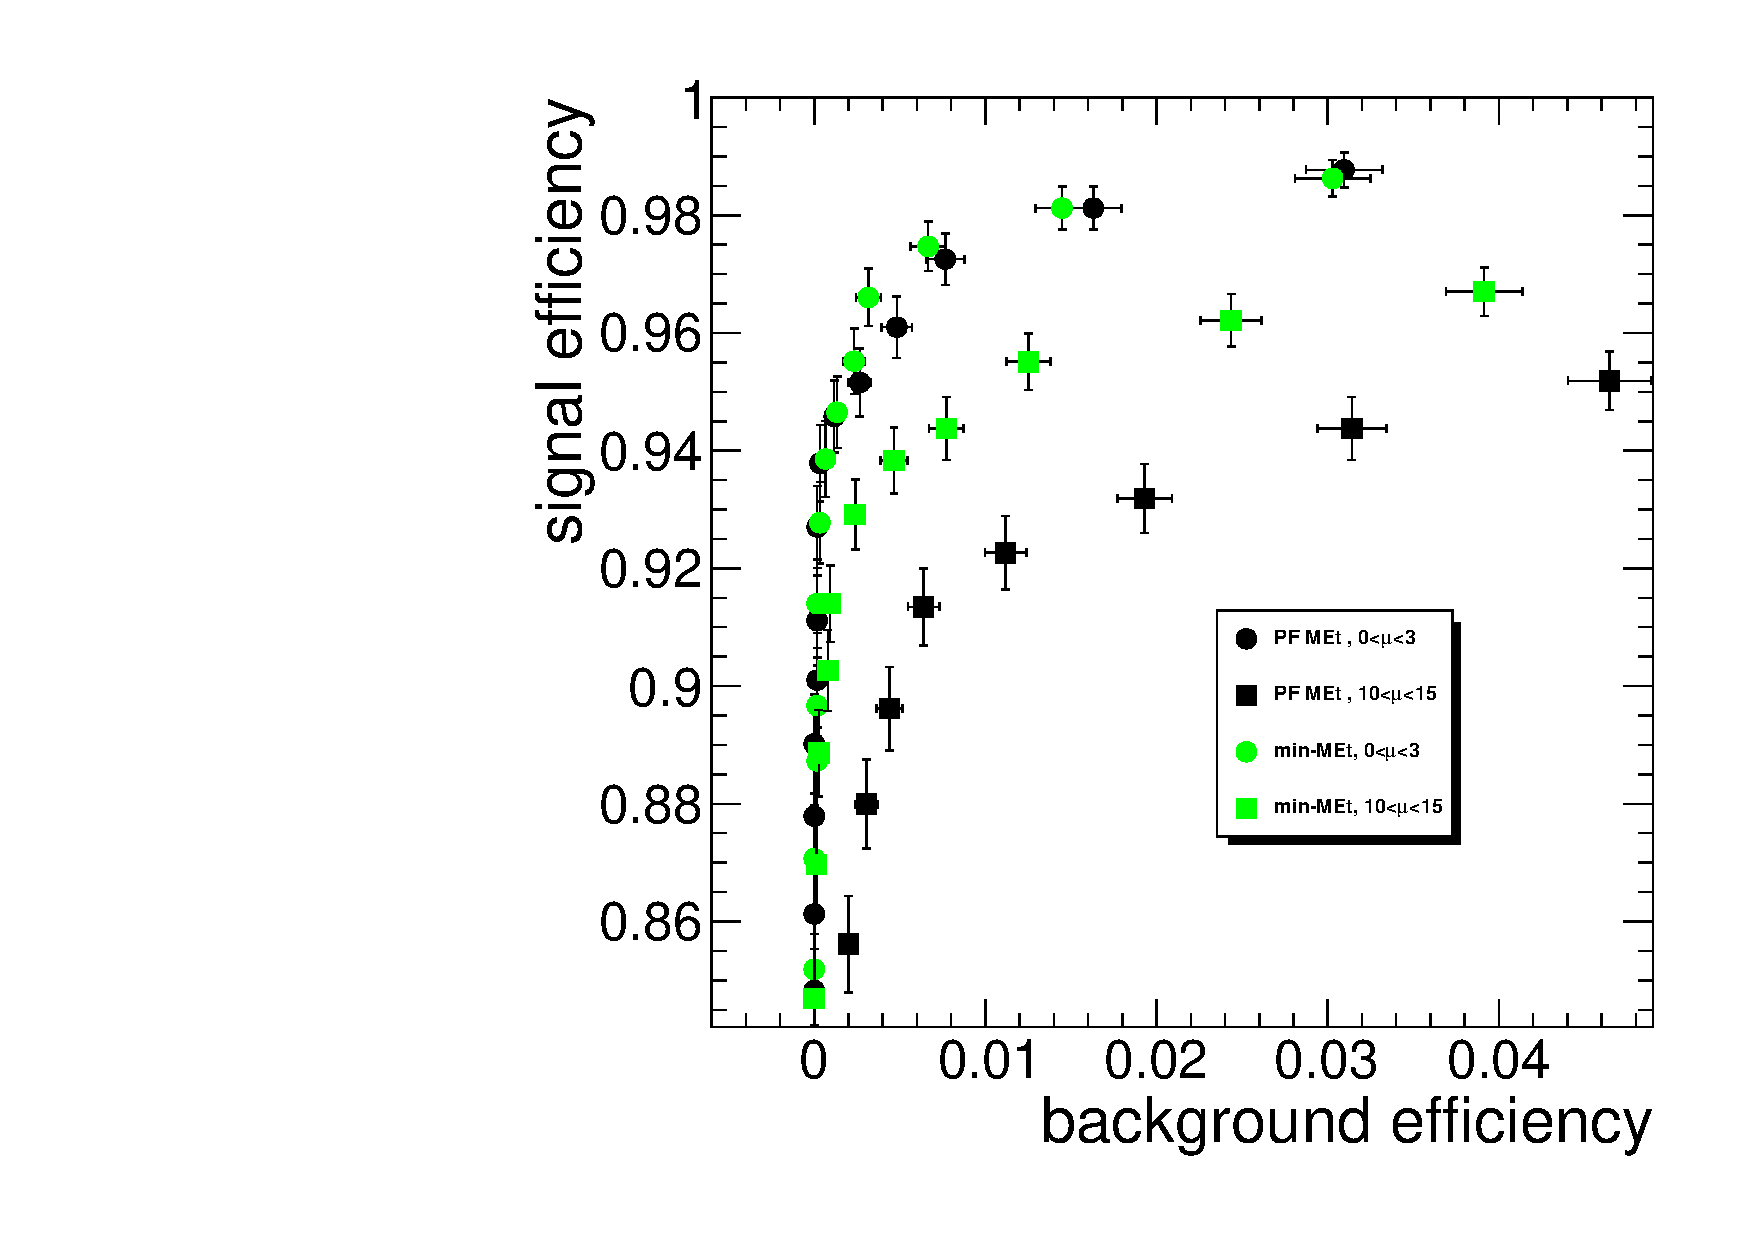
\includegraphics[width=0.45\linewidth]{figures/SignalVsBkgrEfficiency.pdf} 
\caption{\label{fig:met_eff}\protect Left plot shows the efficiency to satisfy
 the requirement pfmet$>$X~GeV as a function of the number of reconstructed 
vertices for Z-events in data and MC. Right plot shows the signal efficiency 
vs. background efficiency, evaluated for H$_{130}$ and DY MC.}
\end{center}
\end{figure}
